
\documentclass{article}
%\usepackage[cyr]{aeguill}
\usepackage[utf8]{inputenc}
\usepackage[T1]{fontenc}
\usepackage[francais]{babel}
\usepackage{amsmath}
\usepackage{fancyhdr}
\usepackage{amsfonts}
\usepackage{makeidx}
\usepackage{caption}
\usepackage{subcaption}         
\title{Implémentation de l'algorithme du fast-marching pour la résolution d'un labyrinthe}
\usepackage[pdftex]{graphicx}
\author{Jean Prost \and Lucas Potin \and Edouard Gouteux}

\begin{document}
	
\maketitle
	
\section{L'algorithme du fast marching}

La méthode du fast marching a été introduite par James Setian. Cette méthode possède notamment des applications en mécanique des fluides et en traitement d'image. Cette méthode permet de résoudre l'équation d'Eikonal, de la forme :
\begin{equation}
|\nabla T|=\mathcal{F}
\end{equation}
Ici, $ \mathcal{F}$ et $T$ sont des fonctions $\mathbb{R}^n \to \mathbb{R}$, ou $n$ peut prendre la valeur 1, 2, où 3. $\mathcal{F}$ est la métrique donné du problème, et $T$ est la fonction à déterminer, avec comme condition initiale $T(x_0) = 0$. Ici nous nous concentrerons sur des fonctions $ \mathcal{F}$ et $T$ de $\mathbb{R}^2 \to \mathbb{R}$ :
\begin{equation}
|\nabla T(x,y)|=\mathcal{F}(x,y)
\end{equation}


\section{Programmation}

\section{Application à la recherche du plus court chemin dans un labyrinthe}
\subsection{Première approche}
On cherche à trouver le plus court chemin pour aller d'un point a à un point b dans un labyrinthe. Le labyrinthe nous est donné comme une image en noir blanc. Tout d'abord on normalise l'image : aux pixels blanc (où l'on peut passer) on affecte la valeur 1, aux pixels noir (que l'on ne peut pas franchir), on affecte la valeur 0. On construit ensuite notre métrique $W$ à partir de l'imager normalisé $I$, tel que pour tout pixel $ij$
\begin{equation}
W_{ij}  = \frac{1}{\epsilon+I_{ij}}
\end{equation}
Cette métrique pénalise donc les passages par les sommets infranchissables. La valeur$\epsilon$ au dénominateur permet d'éviter les divisions par zéro.
On applique ensuite l'algorithme du fast marchinq pour cette métrique, en choisissant comme point initiale l'entrée du labyrinthe. On obtient alors la fonction $T$ représentant la distance à notre sommet initial par rapport à la métrique W (voir figure \ref{fig:Tfm1})

\begin{figure}[h]
	\centering
	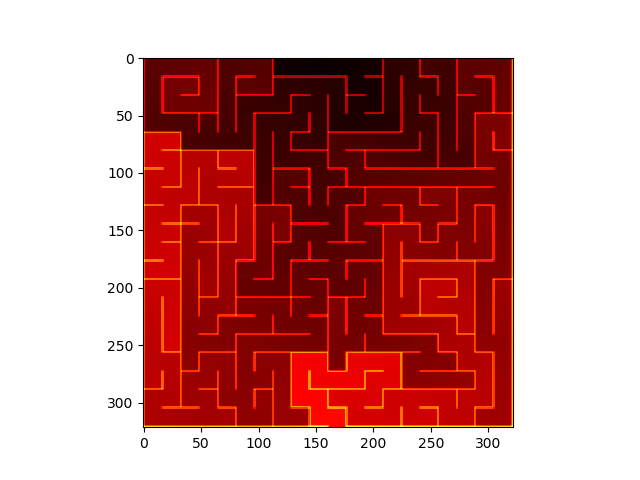
\includegraphics[scale=0.55]{../result/maze_T.png}
	\caption{distance au sommet initial (en haut au centre)}
	\label{fig:Tfm1}
\end{figure}

L'obtention du chemin nous est alors donné en appliquant la descente du gradient sur la fonction T obtenue, en partant de l'autre extrémité du labyrinthe (celle que l'on n'a pas utilisé comme sommet initial). Le chemin corresponds alors à la suite des points obtenus au cours des itérations successives de la descente (voir figure \ref{fig:sol_fm1})

\begin{figure}[h]
	\centering
	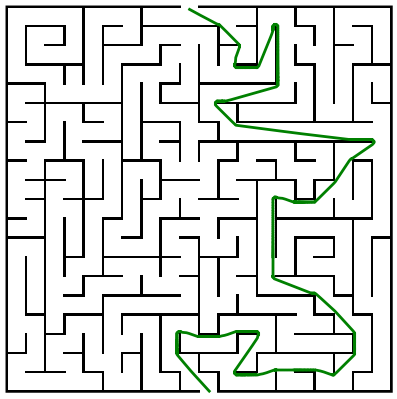
\includegraphics[scale=0.55]{../result/geo_maze.png}
	\caption{Solution du labyrinthe obtenue avec la descente du gradient}
	\label{fig:sol_fm1}
\end{figure}

\subsection{2 fois plus de fast marching!}
Le chemin obtenu est correcte, néanmoins il a tendance à "coller" les bords. Cela n'est pas très beau visuellement, et, pour certaines applications cela peut être problématique. Par exemple, dans le cas de la planification du chemin d'un robot, on peut souhaiter  que notre robot ne passe pas trop près des bords. Pour remédier à ce problème, une solution est d'inclure dans la métrique $W$ une pénalité pour les passages près des bords. Pour cela il faut re en mesure de mesurer la distance d'un point du labyrinthe à son bord le plus proche. L'algorithme du fast-marching nous permet justement de réaliser cette opération. Pour cela on effectue l'algorithme en choisissant comme sommets initiaux l'ensemble des bords du labyrinthe. On appellera la solution obtenue S (speed), dans le sens où, plus la distance au bord sera importante, plus l'on pourra se déplacer au rapidement (figure \ref{fig:Sfm2}) 

\begin{figure}[h]
	\centering
	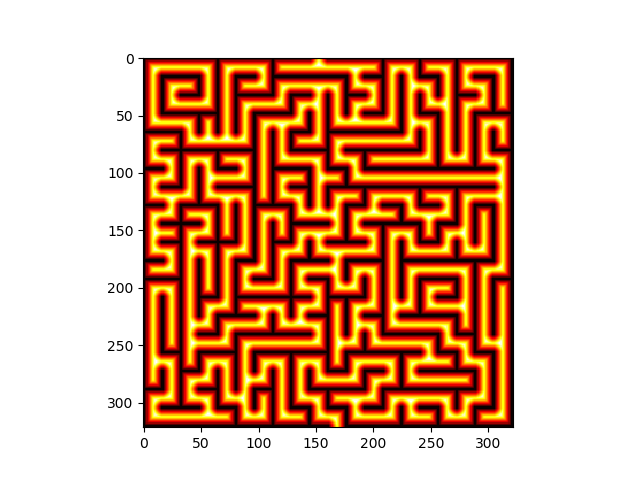
\includegraphics[scale=0.7]{../result/maze_S.png}
	\caption{Distance aux bords, en initialisant l'algorithme avec les sommets correspondants aux bords}
	\label{fig:Sfm2}
\end{figure}

Une fois la fonction S calculé, nous réapliquons l'algorithme du fast-marching, en ajoutant à notre métrique $W$ un facteur prenant en compte la distance au bord :
\begin{equation}
W_{ij} = \frac{1}{\epsilon+I_{ij}} + \alpha*\frac{1}{\epsilon+S_ij}
\end{equation}

Le paramètre $\alpha$ nous permet de choisir l'importance de la pénalisation des passages près des murs. Plus le paramètre $\alpha$ sera important, plus le chemin trouvé sera éloigné des murs. Si on prend $\alpha=0$, alors on retrouve le chemin obtenu avec la première méthode (figure \ref{fig:comp_alpha}).

\begin{figure}
	\centering
	\begin{subfigure}[b]{0.3\textwidth}
		\centering
		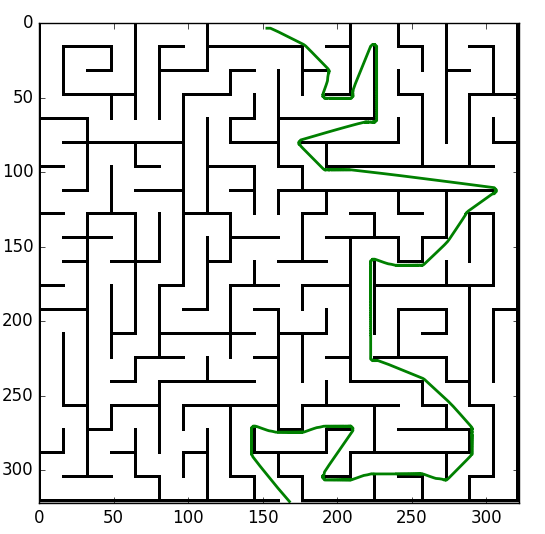
\includegraphics[width=\textwidth]{../result/maze_C0.png}
		\caption{$\alpha=0$}
		\label{fig:y equals x}
	\end{subfigure}
	\hfill
	\begin{subfigure}[b]{0.3\textwidth}
		\centering
		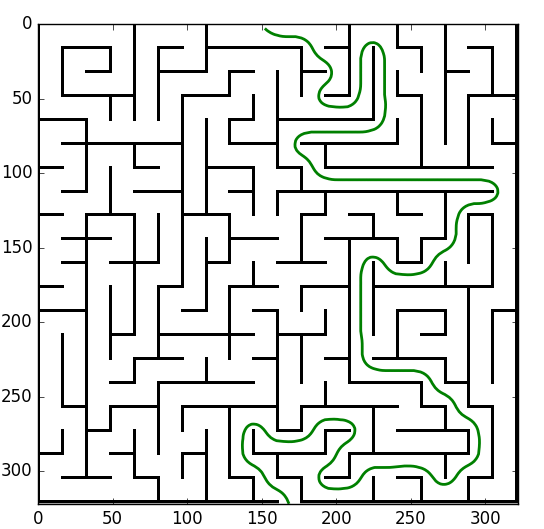
\includegraphics[width=\textwidth]{../result/maze_C05.png}
		\caption{$\alpha=0.5$}
		\label{fig:three sin x}
	\end{subfigure}
	\hfill
	\begin{subfigure}[b]{0.3\textwidth}
		\centering
		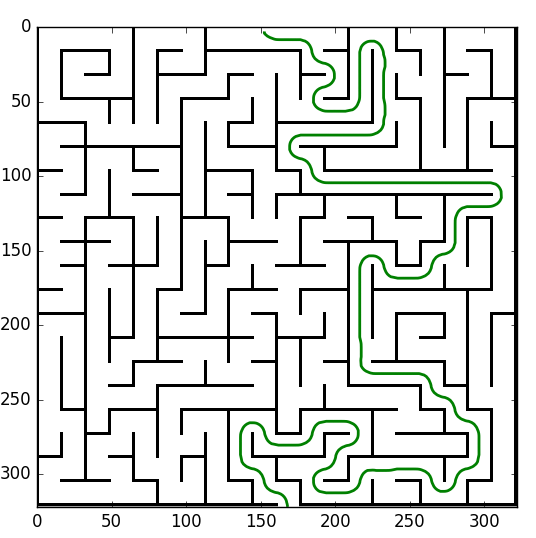
\includegraphics[width=\textwidth]{../result/maze_C10.png}
		\caption{$\alpha=10$}
		\label{fig:five over x}
	\end{subfigure}
	\caption{Influence du choix du paramètre alpha sur le chemin obtenu}
	\label{fig:comp_alpha}
\end{figure}

\subsection{Autres labyrinthes}

 \begin{figure}
 	\begin{center}
 		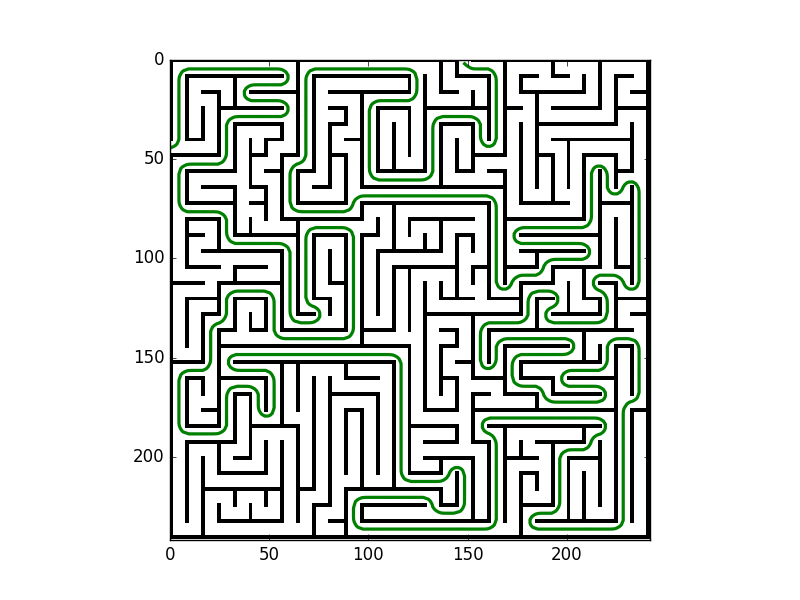
\includegraphics[scale=0.6]{../result/maze3_C.png}
 	\end{center}
 \end{figure}
 \begin{figure}
 	\begin{center}
 		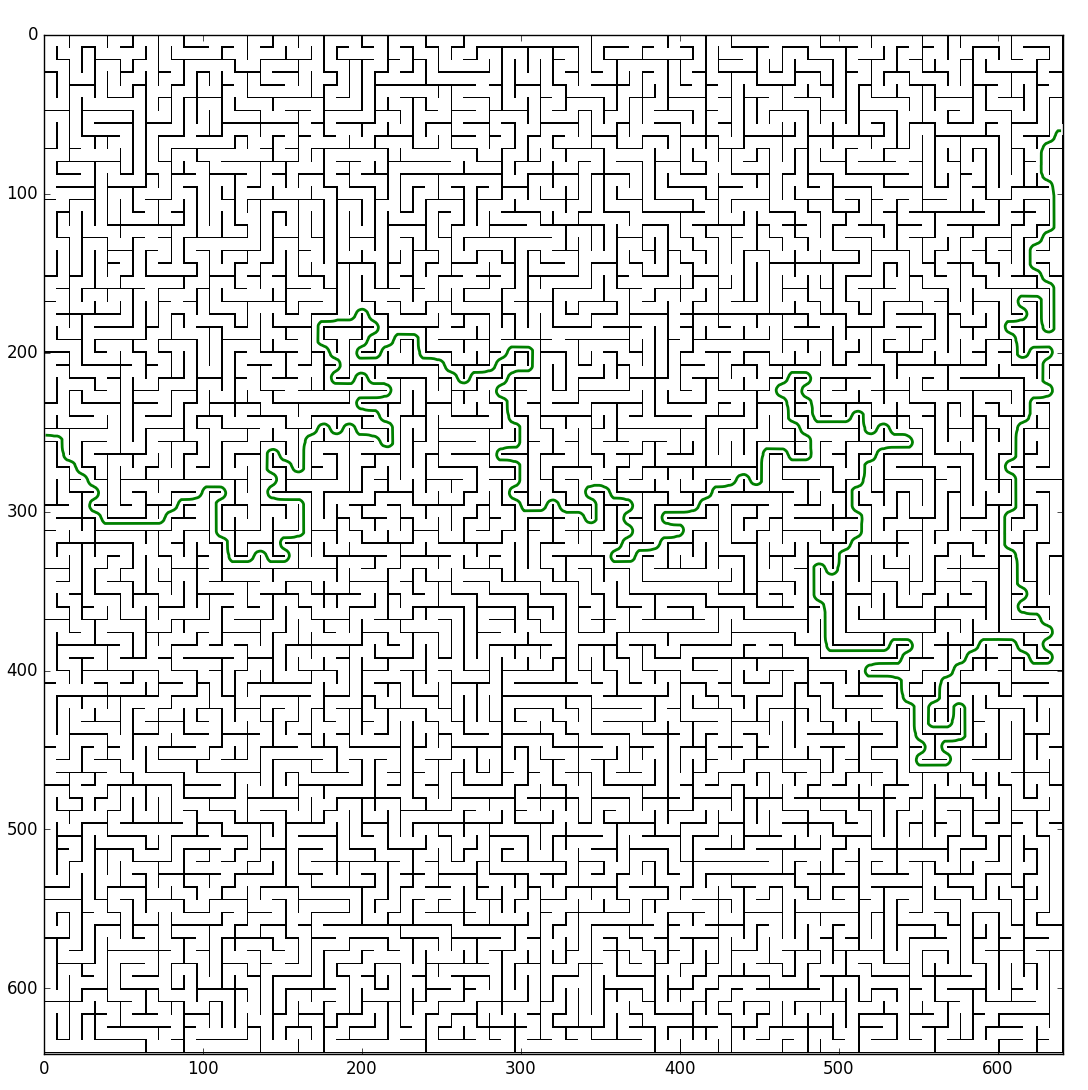
\includegraphics[scale=0.3]{../result/maze5_C10.png}
 	\end{center}
 \end{figure}
 \begin{figure}
 	\begin{center}
 		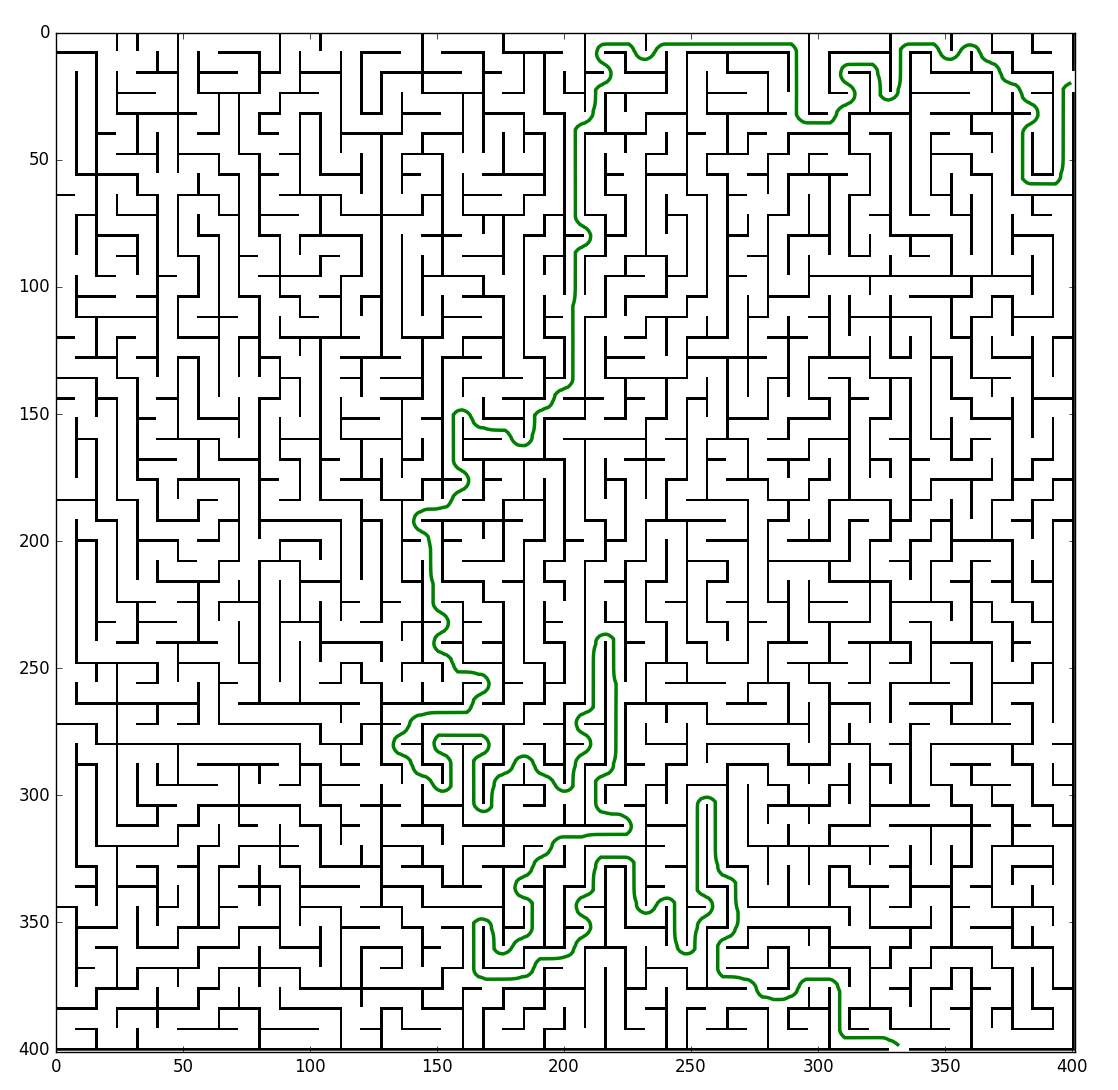
\includegraphics[scale=0.3]{../result/maze6_C.png}
 	\end{center}
 \end{figure}

\end{document} 